% ===== 第五章 问题四：螺距1.7 盘入 + S形调头 + 中心对称盘出（约4-5页） =====
\section*{五、问题四：螺距 1.7 m 的盘入、调头与盘出}

\subsection{问题设定}
螺距 $p=1.7$m（$a=1.7/(2\pi)=0.270563$\,m/rad）。龙头沿螺线盘入，进入以螺线中心为圆心、半径 $4.5$m 的调头空间，做 S 形调头后，沿与盘入螺线关于螺线中心中心对称的盘出螺线盘出。要求给出 $-100\thicksim100$s 整队位置速度与指定节点表，并讨论调头圆弧可否缩短。[C4,C8]

\subsection{复合路径的几何构造}
设盘入螺线为 $P(\theta)=a\theta(\cos\theta,\sin\theta)$，中心对称盘出螺线为 $-P(\theta)$。入口 $E$ 位于盘入螺线 $r=4.5$m 边界（$\theta_E=4.5/a=16.632$rad），出口 $X=-E$ 位于盘出螺线同样 $r=4.5$m。复合路径为：

\[
\text{盘入螺线 }(\theta:\ 100\downarrow \theta_E)\ \to\ \text{S形调头}\ \to\ \text{盘出螺线 }(\theta:\ \theta_E\uparrow 100),\qquad X=-E.\
\]

\textbf{S 形调头}由两段相切圆弧组成，前段半径 $R_1$ 为后段 $R_2$ 的 2 倍，且两圆弧分别与盘入、盘出螺线相切：
\begin{equation}\label{eq:sarc}
R_1=2R_2,\qquad R_2=1.5027\ \text{m},\quad R_1=3.0054\ \text{m},\quad \Delta=3.0215\ \text{rad}.
\end{equation}
其中 $R_2$ 由“两圆弧外切 + 前段切盘入螺线于 $E$ + 后段切盘出螺线于 $X$”的数值约束求解（详见执行日志）。[log:q4.R1, q4.R2, q4.turn\_arc\_angle\_each]

调头圆弧长度为
\begin{equation}\label{eq:lturn}
L_{\rm turn}=R_1\Delta+R_2\Delta=3R_2\Delta=3\times1.5027\times3.0215=13.621\ \text{m}.
\end{equation}
数值验证：S形调头圆弧全程 $r\le4.5$m（最大半径 4.500m），恰好位于调头空间内。[log:q4.turn\_arc\_len, q4.turn\_arcs\_max\_r, q4.turn\_fits]

龙头沿复合路径按弧速 1 m/s 行进；把手 $i$ 位于龙头前把手弧长 $u_{\rm head}-D_i$ 处。入口弧长 $u_E=1315.468$m，复合路径总长 2644.557m。[log:q4.uE, q4.composite\_total\_len]

\subsection{求解与碰撞检查}
对 $-100\thicksim100$s 逐秒布置 224 个把手并作板段自交扫描：全区间零碰撞（$collision\_free=True$），最小相邻把手间距 $1.5683$m。图 \ref{fig:q4path} 给出复合路径，图 \ref{fig:q4gap} 给出全程最小相邻间距随时间的变化（不低于 1.57m）。[log:q4.collision\_free\_q4, q4.min\_adjacent\_handle\_gap]

\begin{figure}[H]\centering
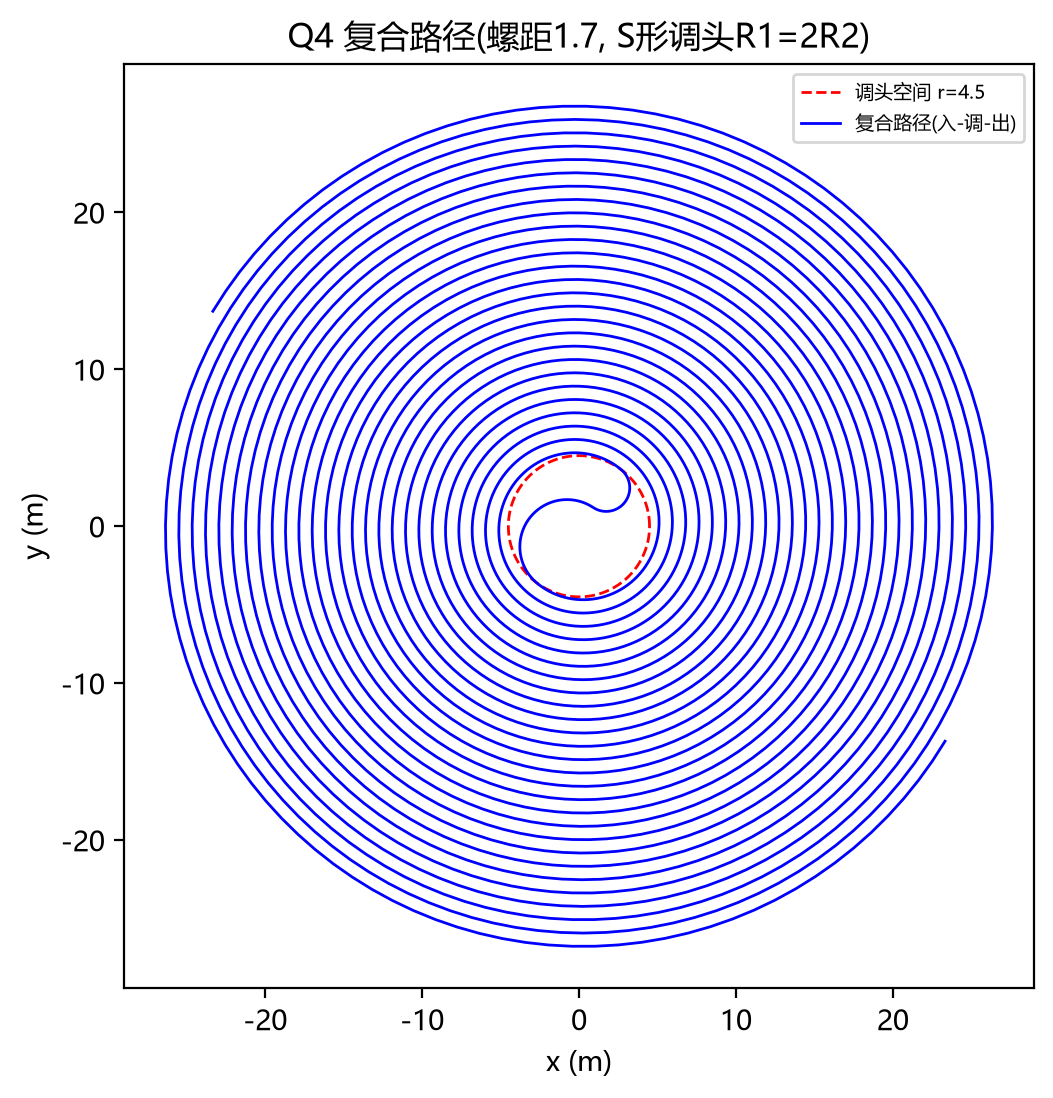
\includegraphics[width=0.72\textwidth]{../artifacts/figures/fig4_q4_path.png}
\caption{问题四：复合路径（盘入—S形调头—中心对称盘出），调头空间红虚线[log:q4]}
\label{fig:q4path}
\end{figure}

\begin{figure}[H]\centering
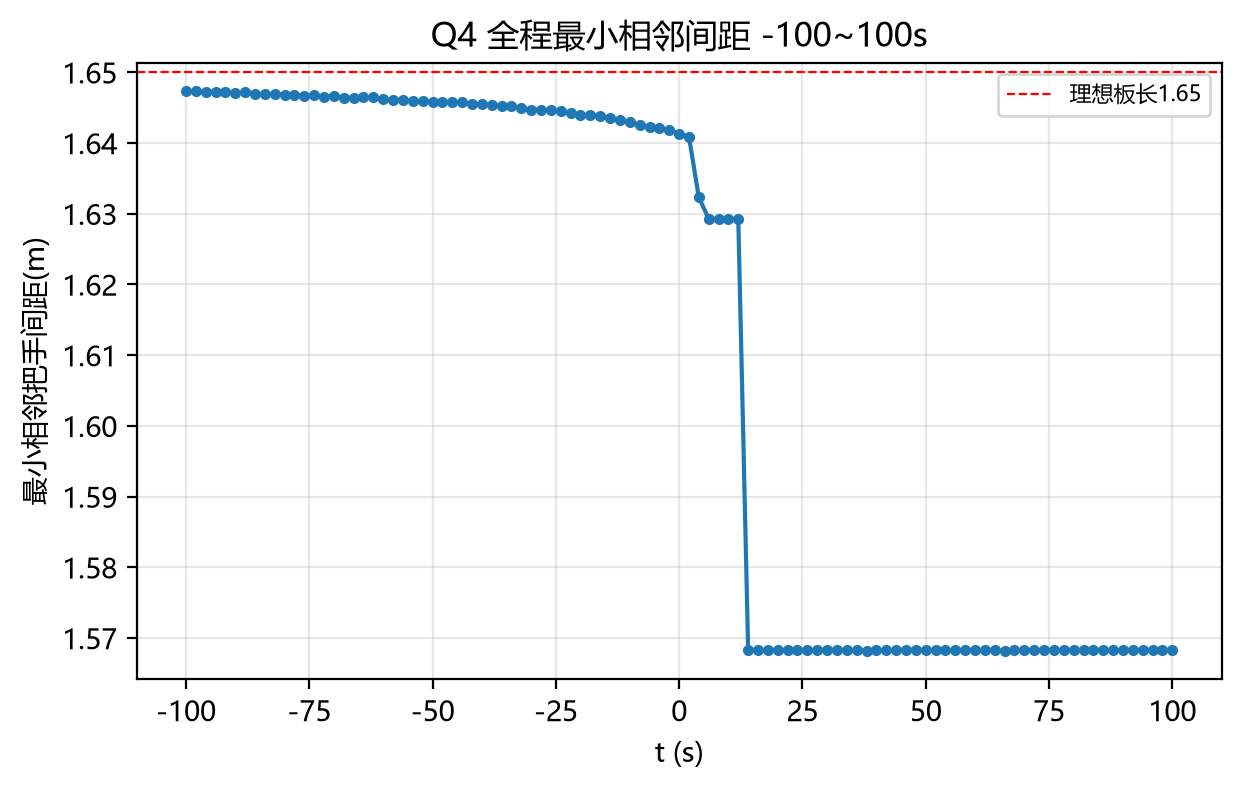
\includegraphics[width=0.82\textwidth]{../artifacts/figures/fig6_q4_spacing.png}
\caption{问题四：$-100\sim100$s 全程最小相邻把手间距[log:q4.min\_adjacent\_handle\_gap]}
\label{fig:q4gap}
\end{figure}

\subsection{指定节点表}
表 \ref{tab:q4} 给出 $-100/-50/0/50/100$s 龙头前把手位置、各指定节前把手与龙尾后把手位置（详见 $result4.xlsx$ 与执行日志）。[log:q4.paper\_sample]

\begin{table}[H]\centering\small
\caption{问题四指定时刻龙头前把手与龙尾后把手位置[log:q4.paper\_sample]}
\label{tab:q4}
\begin{tabular}{ccrr}
\toprule
时刻 & 节点 & $x$ (m) & $y$ (m) \\
\midrule
$-100$s & 龙头前 & 7.771393 & 3.728394 \\
$-100$s & 龙尾后 & $-1.232604$ & $-16.506292$ \\
$-50$s & 龙头前 & 6.605791 & 1.904929 \\
$-50$s & 龙尾后 & 0.496911 & 15.702755 \\
$0$s & 龙头前 & $-2.711856$ & $-3.591078$ \\
$0$s & 龙尾后 & $-2.414163$ & $-14.627153$ \\
$50$s & 龙头前 & 1.327366 & 6.175077 \\
$50$s & 龙尾后 & 6.703938 & 12.162073 \\
$100$s & 龙头前 & $-3.167139$ & 7.542052 \\
$100$s & 龙尾后 & $-11.461372$ & $-5.863948$ \\
\bottomrule
\end{tabular}
\end{table}

\subsection{调头圆弧可否缩短}
调头路径弧长 $L_{\rm turn}=3R_2\Delta$，随 $R_2$ 线性增长，因此减小 $R_2$ 可缩短调头路径。[log:q4.can\_shorten] 但 $R_2$ 存在下限：两圆弧须满足 $R_1=2R_2$ 且与两条螺线相切，并全部位于 $r\le4.5$m 调头空间内。本文取满足相切约束的临界构造（$R_2=1.5027$m，$R_1=3.0054$m，恰好撑满 $r\le4.5$），故该取值已是该约束族下的紧凑解；进一步缩短需放宽“全程 $r\le4.5$”或相切刚性，属工程权衡。

\subsection{本章小结}
问题四在螺距 1.7m 下构造并验证了“盘入—S形调头—中心对称盘出”复合路径，$R_1=2R_2$（$3.0054$/$1.5027$m）两圆弧与两螺线相切且处于调头空间内，全程 $-100\sim100$s 零碰撞、最小间距 1.5683m。调头路径随 $R_2$ 线性缩短，本文取相切约束下的紧凑解。